 \documentclass[11pt,twoside,a4paper]{book}   
\usepackage[czech, english]{babel}
\usepackage[T1]{fontenc}
\usepackage[utf8]{inputenc}
%=-=-=-=-=-=-=-=-=-=-=-=--=%
\usepackage{lmodern}
\usepackage{graphicx}
\usepackage{k336_thesis_macros}
\usepackage{pdfpages}
\usepackage{afterpage}
\usepackage[super]{nth}
\usepackage{array}
\usepackage[capitalise,noabbrev,nameinlink]{cleveref}

\usepackage{nomencl}
\makenomenclature

\usepackage{amsthm}
\newtheorem{definition}{Definition}[chapter]

\newcommand\TypeOfWork{Master's Thesis}   \typeout{Master's Thesis} 
\newcommand\StudProgram{Open Science}
\newcommand\StudBranch{Data Science}

\newcommand\WorkTitle{Problem detection and prediction in complex software architectures}
\newcommand\FirstandFamilyName{Bc. Ondřej Borovec}
\newcommand\Supervisor{Ing. Martin Svatoš}

\usepackage[
pdftitle={\WorkTitle},
pdfauthor={\FirstandFamilyName},
bookmarks=true,
colorlinks=true,
breaklinks=true,
urlcolor=blue,
citecolor=blue,
linkcolor=blue,
unicode=true,
]
{hyperref}


\usepackage{color} 
\newcommand{\ms}[1]{\textcolor{red}{#1}}

\begin{document}

\baselineskip=16pt plus1pt

\typeout{************************************************}
\typeout{Language: english}
\typeout{Type of Work: \TypeOfWork}
\typeout{Study Program: \StudProgram}
\typeout{Study Branch: \StudBranch}
\typeout{Author: \FirstandFamilyName}
\typeout{Title: \WorkTitle}
\typeout{Supervisor: \Supervisor}
\typeout{***************************************************}
\newcommand\Department{Department of Computer Science and Engineering}
\newcommand\Faculty{Faculty of Electrical Engineering}
\newcommand\University{Czech Technical University in Prague}
\newcommand\labelSupervisor{Supervisor}
\newcommand\labelStudProgram{Study Programme} 
\newcommand\labelStudBranch{Field of Study}


%%%%%%%%%%%%%%%%%%%%%%%%%%    Titulni stranka / Title page 

\coverpagestarts

%%%%%%%%%%%%%%%%%%%%%%%%%%   Assignment

\includepdf[pages={1}]{blankPage.pdf}

\includepdf[pages={1}]{blankPage.pdf} % English Assignment

\includepdf[pages={1}]{blankPage.pdf}

\includepdf[pages={1}]{blankPage.pdf} % Czech Assignment

%%%%%%%%%%%%%%%%%%%%%%%%%%%    Podekovani / Acknowledgements 

\acknowledgements
\noindent
Zde můžete napsat své poděkování, pokud chcete a máte komu děkovat.


%%%%%%%%%%%%%%%%%%%%%%%%%%%   Declaration 

\declaration{In Prague on November 30, 2018}


%%%%%%%%%%%%%%%%%%%%%%%%%%%   Motivation

\chapter*{Motivation}

\ms{Takové zvláštní mít toto ještě před abstraktem a kompletně mimo všechny sekce. Hodil bych to spíš do první kapitoly úvod / motivace / \dots}

During my studies I had an internship and later a regular job as a DevOps Engineer. The team, I was part of, is responsible for running a big cluster of NoSQL storage with surrounding infrastructure in multiple separated zones of the world as an internal logging platform. You can definitely image\ms{,} we were facing some problems nearly every day and more than an DevOps Engineer I felt as a PostOps when we were trying to figure out the root cause of the problems. It was never easy, because during the down-times of our service we were under a big pressure going though log files and running several analysis tools.

At the time we would give nearly everything to have a reliable solution which would warn us in advance so we had more time to react. But we were not satisfied with any existing solution around. Since we were dealing with structured data and time series, my main field of study - Applied machine learning comes really handy. So, when I started to think about my master thesis this was the natural choice, because I wanted to work on something I know and from what others could benefit as well.

\vspace{20mm}
\begin{flushright}
Ondrej Borovec
\end{flushright}

%%%%%%%%%%%%%%%%%%%%%%%%%%%%    Abstract 
 
\abstractpage

English abstract

\abstractpage

Czech abstract

%%%%%%%%%%%%%%%%%%%%%%%%%%%% Notation

\printnomenclature
\nomenclature{$[..]$}{Tuple of values.}
\nomenclature{${..}$}{Set of values.}

%%%%%%%%%%%%%%%%%%%%%%%%%%%%    Content tables

\tableofcontents
\listoffigures
\listoftables

%**************************************************************

\mainbodystarts
\normalfont
\parskip=0.2\baselineskip plus 0.2\baselineskip minus 0.1\baselineskip

Modern high demands on IT industry cannot be satisfied with a one-program single solution any more. Current software architectures rely on multiple part solutions of many other vendors which are combined to solve new problems. We think, it can be said, that most of software products you can find on the market, both open source as commercial, are really reliable with minimum run-time failures, otherwise they would lose their position and reputation. Plus the is a new common rend, that programs are becoming self-healing, so it a problem occurs, it finds a way how to reach a stable state on its own for instance as describes this Google patent \cite{khan2011self}. But developers can only focus on their own products, so if you are designing your service using these products which are relying on each other and also the effect of non-laboratory environment (network latency and unreliability, limited memory and machine resources, ...) can cause unpleasant troubles.

Every down time of a service comes along with consequences which can be in a form of a money penalization, losing of user preferences of data consistency problem. None of these is good for a company so every service owner has to have some people, DevOps engineers of System administrators, who are taking care of his service and who can immediately react if some failures are observed. Such person then have to investigate what is the root cause of an incident, most often by viewing related program log files and then has to d appropriate action to make system running correctly. You can be sure, that somebody had dealt with exactly the same of very similar problem, so it is possible to google a solution, but to do that, you need all related system and software information to identify the problem similarity. Such investigation is not an easy task, it is always hard to determinate which all components took a part at the incident.

In this paper we would like to identify the challenges of this problematic in Section \ref{sec:problemStatement}. The main focus is payed at to failure prediction and early detection and also to solution suggestion, so service maintenance can be maximally automated. Section \ref{sec:currentSolution} lists most important current frameworks and real implementations which are heaping to automate service operations, We are also trying to compare all mentioned solution and highlight current weak sides of them. Then we proposed our framework idea which take the best of all existing solution, combine them all together using our point of view on the problematic. Please keep in mind, this our solution has never been implemented yet and it is only a general idea.

\chapter{State of the art}
\label{chap:stateOfTheArt}

General anomaly detection is very wide field since the concept is applicable with just slight adaptations to nearly every field of human interest. There are hundreds of papers which are proving how useful is to detect and know about an anomaly in various areas, but it has also been shown every algorithm is more effective and successful in an area with strict rules. It means, deterministic computer and software field are excellent candidates.

Even with the deterministic space of applications and software in general it is not easy to detect anomalies. Operators who were in charge of that up to recent time had to have good knowledge to the system they are taking care of to be able to correctly understand produced time series and logs. This is the main reason why there is no 100\% efficient general approach or tool so far.  In this chapter we will discuss most of the current frameworks and practises for anomaly detection in software field.

From time to time, it is more interesting to know the reasoning behind and problem than the detection itself. We all know the famous phrase from the series IT crows: "\textit{Have you tried turning it off and on again?}" Most of the members of IT crowds will agree that it is most often the best and easiest way to fix anything, but if you do not know why it happened, it may cause some problems again. So, we will try to always discuss the potential of reasoning for every method listed below.

The amount of software solutions has increase radically over the past several years. It goes hand in hand with the amount of software projects which are meant to make all the related work easier. A lot of them are designed to deal with software architecture maintenance and monitoring, but their usage may be confusing for users.

In this chapter we will cover time series analysis and anomaly detection principles along interesting methodologies related to logging, log collection and log storing as well as open source frameworks and commercial bounded to this IT architecture analysis. In this chapter we would like to highlight the most interesting concepts which are currently used and, mainly, the ones which are related to our future work. Even though we will also discuss general techniques we will do my best to relate everything to the field of interest of this thesis - complex software architectures.

Most of the content of this chapter is not vital for understanding the technicalities of our contribution. It servers mostly as an overview to anybody who does not have a deep knowledge of general anomaly detection aw well as who is interested in current results of software anomaly detection. If you desire, you may skip this chapter and continue to chapter \ref{chap:dataset} or chapter \ref{chap:solution} which are more related to our work.


\section{Software logging and reliability}

There are many different types of software, it starts with a single stand-alone desktop application and reaching the sky with cloud application connecting all kinds of wearable devices. All the applications differ in features, target usage and scale, but we can still identify some features which are common to all of them. The one we would like to highlight and have as ground truth to our work is that every application and architecture is deterministic and the only indeterminism is brought by an internet unreliability, hardware failure, system termination signal or others belonging to the same category.

This is an important statement, because during our discussions with many professionals in this field there was frequently asked this question: "Do we really need a research and machine learning tool for program logs since all programs are supposed to be deterministic?" We have to agree, this is a good question. But an application would be deterministic under the condition we know all potential aspects which can affect its run. And there is no chance we can stream such collection of information about every application with current possibilities.

This requirement becomes even more unreachable considering cloud applications. For such application also we should, definitely, keep in mind following requirements and best practice design:

\begin{itemize}
    \item An architecture for a cloud application consists from micro services - it means there are multiple teams and projects which all are developed independently and are delaying with just small problems. The problem is that the is luck of deep cooperation between such micro services if one has a problem other does not have to know it.
    \item Such application has to be able to scale - it runs on multiple machines in different countries. This is mostly related to already mention problem of potential unreality of the internet. You can argue with potentially better protocols, but there is currently no way to ensure full steadiness.
    \item In the modern age, many teams and companies are abandoning standard version releasing in favour of continuous deployment, blue-green deployment, canary releasing and AB testing. It means, everybody can witness different states and behaviour cross same micro services.\footnote{\url{http://blog.christianposta.com/deploy/blue-green-deployments-a-b-testing-and-canary-releases/}}
\end{itemize}
Keeping everything in mind, we can, definitely, say, being in charge of keeping a cloud application stable, health and alive, can be a heroic task from time to time. This is also one of the main reasons we choose to work on this topic to make life of such people easier and to try automating most of the process.

\subsection{Logging techniques}
\label{ssec:sota_logging_logging}

Application logging is not a mandatory feature, but it is, definitely, part of best practises to record runtime behaviour. Otherwise there is just a really narrow opportunity for anybody to be able to debug a running application or identify a potential problem. On the other hand, logging has been part of application development since nearly the beginning. Therefor even the best practice evolved a lot and it makes it easy for developers to implement it. 

We can sum up some best practice rules to every logger - component of an application responsible for logging:
\begin{enumerate}
    \item An application should be logging about itself as much ass possible with each message containing a timestamp of related event and labeled with a standard severity level.
    \item Users should be able to customize logging possibilities of an application they are running.
    \item Preferably use a standard logging library like Log4j, Log4net, boost.log or python logging instead of writing your own. But is should be a framework which a flexible output option.
    \item Every log message should be in format of a patter string with a static and dynamic parts or a standard structure format as yaml or json with a predefined field mapping. The static part of each log message is a free-format string describing a runtime event or a property and the dynamic part is event of moment specific information.
    \item Any action of your logger cannot block application itself for any reason such as inability of creating of a log file or dependent process for printing a message.
\end{enumerate}

But even the best practice rules does ensure the right logging since there are not strict guidelines. There are 3 main questions related to logging topic: "What to log?", "Where to log? and"How to log?". There are important conclusions resulting from these questions, which can significantly influence software performance or disk I/O bandwidth. So, let's take a look at them separately.

\begin{itemize}
    \item \textbf{\textit{What to log?}} - this question is really connect to the point 1 of the best practice rules. It is question what to log on which level to help users maximally understand problems, warning and runtime behaviour. 
    \item \textbf{\textit{Where to log?}} - the other question is about log command placement in a source code. A logging piece of code can be part of each run of a loop on a summary message after it finishes. 
    \item \textbf{\textit{How to log?}} - according to \cite{chen2017characterizing} this the most complex topic about developing, maintaining high quality and overall consistency of logging code. The publication declares logging anti-patterns as recurrent mistakes which may hinder the understanding and maintainability of the logs.
\end{itemize}

Up to now we were more focused at how to implement logging in an application code for better understanding of a reader. But we want to design an automated system, so the first step after reading a message from a log file is to transform it to a format which is understandable for machines and suitable for machine learning. We can also find a term \textit{log key} in \cite{fu2009execution} and \cite{du2017deeplog} which suggested representing a log message by a pattern key based on the free-text constant part of a log followed by vector of variables of that pattern - expecting behaviour described in the \nth{4} point of our best practice rules. This representation also be extended to forget the exact timestamp when a message was printed and transforms to time difference to a previous related log messages. For better understand and illustration take a look at table \ref{table:logParsingKeyLog}.

\begin{table}[h!]
\renewcommand{\arraystretch}{1.2}
\centering
\begin{tabular}{| >{\centering\arraybackslash}m{4cm} | >{\centering\arraybackslash}m{4cm} | >{\centering\arraybackslash}m{1.5cm} | >{\centering\arraybackslash}m{3cm} |} 
 \hline
 Original message & Pattern with wildcard (constant part) & Pattern key & Variable vector (variable part) \\ 
 \hline
 $t_1$ Pipeline stated to operate & Pipeline stated to operate & $k_0$ & [ $t_1 - t_0$ ] \\ 
 \hline
 $t_2$ Delivered 5 messages & Delivered * messages & $k_1$ & [ $t_2 - t_1$, 5 ] \\
 \hline
 $t_3$ Failed connection to server server-1 & Failed connection to server * & $k_2$ & [ $t_3 - t_2$, server-1 ] \\
 \hline
 $t_4$ Failing to connect to server-1 for 10 minutes, connecting to server-2 & Failing to connect to * for * minutes, connecting to * & $k_3$ & [ $t_4 - t_3$, server-1, 10, server-2 ] \\
 \hline 
 $t_5$ Failed connection to server server-2 & Failed connection to server * & $k_2$ & [ $t_5 - t_4$, server-2 ] \\
 \hline

\end{tabular}
\caption{Example of log transformation to log key format}
\label{table:logParsingKeyLog}
\end{table}

Unfortunately, no program or application provides such complex information since this structured format is not human readable. It would be beneficial to have information about all potential logs and its patterns which can be printed into a log file, at this moment we have to find another solution to the problem of transforming a free-text format to more structured format. 

Traditional solution implemented by operators is based on regular expression. The problem is, there is no universal database so every set of regular expressions has to be maintained company by company. Such maintenance is not easy, since software can be developed by hundreds of developers who has different style of logging which results to high number of expressions. Plus, every software is developing with new patterns appearing every release.

Really interesting way is source code analysis. Many projects are now released as an open source which make the source code easily accessible. It is possible to write a script which greps all lines related to logging and parses the patterns as was implemented in \cite{xu2009detecting} for Java, C, C++ and Python in 2009. A disadvantage is that the source code has to be known prior log analysis and also not every application provides access to the code. 

Another solution for log parsing problem - LCS - is more suitable for streamed data, to which category logging belongs. An algorithm using Longest common subsequence is described in \cite{fu2009execution} with accuracy higher than 95\%. The procedure is even improved in \cite{du2016spell} by prefix trees. The potential problem here may be similarities of multiple nodes in a same cluster where ip addresses may start with same numbers. \cite{he2016evaluation} states that log pre-processing based on domain knowledge can significantly increase log parsing efficiency. For instance removing domain or node names starting with environment name by a hash or removing IP addresses.

The last one we would like to list here is approach introduced in Drain \cite{he2017drain}. The system is using log message filtering based on number of tokens and a limited number of first tokens which are supposed to be part of constant parts of logs. The potential weakness of hat approach is possibility of placing unstable number of tokens as one variable, but it is not often observed behaviour. 

We can say, there are many ways how to implement logging as well as ways how to process such logs when there are stored in a file. Used technology will differ form and architecture to an architecture, but the concept we want to present in this thesis has to be as universal as possible.

Table \ref{table:logParsingFrameworks} shows some currently available framework for log parsing in online and offline mater with their features and average accuracy based of a test in \cite{he2017drain} and post pre-processing results in \cite{he2016evaluation}.

\begin{table}[h!]
\centering
\begin{tabular}{|c | c | c | c | >{\centering\arraybackslash}m{3cm} |} 
 \hline
 Framework & Release year & Methodology & Training & Average accuracy in \cite{he2017drain}/ in \cite{he2016evaluation} \\ 
 \hline
 LKE \cite{fu2009execution} & 2009 & clustering & offline & 0.608 / 0.6625 \\ 
 \hline
 IPLoM \cite{makanju2009clustering}& 2009 & heuristic based & offline & 0.894 / 0.8825 \\
\hline
LogSig \cite{tang2011logsig}& & clustering & - & - / 0.9425\\
\hline
SLCT \cite{vaarandi2003data}& 2003 & heuristic & - & - / 0.9125 \\
 \hline
 SHISO \cite{mizutani2013incremental}& 2013 & trees & online & 0.772 / - \\
 \hline
Spell \cite{du2016spell}& 2016 & LCS & online & 0.906 / - \\
 \hline 
Drain \cite{he2017drain}& 2017 & trees & online & 0.934 / - \\
 \hline

\end{tabular}
\caption{Overview of log parsing frameworks}
\label{table:logParsingFrameworks}
\end{table}

\subsection{Machine monitoring}
\label{ssec:sota_logging_monitoring}

Application logging should give you all potential answers about runtime behaviour of an application, but knowing statistics about a machine you are running the application on may give you important insights. This have been proved by \cite{farshchi2015experience} using VM operation logs with machine statistics. There are sever variables which are useful to know:

\begin{itemize}
    \item \textbf{CPU utilization} – Processing power of CPUs is the heart of every computer machine. It can happen that your application consumes all computing resources and then it slows down or even stops working properly. This is the reason why many engineers sets a warning level on CPU usage so then are alert in advance and have time to react. This information and earning can also be beneficial side variable to information contained in logs.
    
    \item \textbf{Memory usage} - Reading and writing directly to RAM is much faster than swapping to the main drive, so most of application are trying not to. Current price development allows us to have memory of a size, developers from 90's could only dream about, but the problem is that our usage grows hand to hand with the size we can effort, so we still have to deal with freeing the memory. It is really language dependent, but for instance lets speak shortly about Java which one of the most common languages used for commercial software. Java application where memory management is fully in hands of a garbage collector can reach a point, where memory us full and processes of the collector blocks the application for couple of minutes. It is true, it does not happen often, since memory if being freed continuously, but there are observed incidents.
    
    \item \textbf{Drive stats} – Since drive size is in general much higher than memory, we do not have to deal with a problem that drive is too small to serve as backup place for overflowing memory, even though it is recommended to have at least couple of gigabytes free for correct and smooth functionally of a server. 
    
    Occupancy of a drive plays more important role for application which are more big data focus such as databases or message brokers. In case a drive is full, such application can start rejecting new incoming documents which can start a snow-ball effect. One more interesting case from the real industry. If your application logging is not correctly set (too low significance level and no log rotation), it may happen that log files occupies more space than actual data you want to store. At that moment it is even better to know the distribution of drive usage than single percentage number of used space.
    
    Another potentially useful but not definitely crucial information about drive is input and output statistics. Reads and writes per second or number of queued instruction can imply problems, but they would be there probably from beginning.  
    
    \item \textbf{Bandwidth, SNMP, HTTP(S) and ping} - In the age of cloud application and services, the internet plays even more significant role than before. Unfortunately the internet is also the most unreliable bottom neck of this list. There are many ways how to monitor the internet, you can have a health check from a remote machine testing attainability or have local tests for connection speed. Any early warning flag is useful.  
    
    \item \textbf{Internal system events} - Every server has its operation system under which roof applications are running. Since OS - application is parent - child relation, there is a big high chance that system action cause reaction in application. Another thing is that we can be able to identify user actions and distinguish standard operations from others.  So, for example do not trigger an alert after planned restart.
\end{itemize}

There are definitely more variables which can be tracked, we decided to list only the ones which seems to be the most important to us 
\subsection{Current problem detection practise}

Architecture owners and operators are ingesting a lot of time developing scripts and tools which would free them from tracking all log files and time series to keep everything running. But still there are many companies around which do not implement event the basic principles.

Understanding of software runtime behaviour though logging is getting harder and harder with every new modern architecture introduced. We can identify some main challenges of logging within complex software architectures:

\begin{itemize}
    \item \textbf{Complexity} is closely related to our definition of complex software architecture \ref{def:complexSoftwareArch}. Microservices and subsolutions are more and more dependent on each other and it is not easy to uncover the dependency map. 
    \item \textbf{Volume} and amount of logs are scaling as their service grow. To serve millions of users, you need to have hundreds of machines with even more running programs and each of them are generating their own logs. \cite{mi2013toward} in 2013 worked with large scale service which produced about 50GB of logs per hours, but in chapter \ref{chap:dataset} we will show that the amount can be even higher for current standalone service.
    \item \textbf{Accuracy} especially false positive rate can be overwhelming in case we want to be sure, no anomaly is missed. On the other hand, alerting every state which is just slightly suspicious can easily overwhelm an operator and in the end such alerting system is little to useful. 
    \item \textbf{Online processing } is undiscussable mandatory feature for every alerting system. If warning are not timely in order and warning are delivered before or at least at the time when it happened, there is really no use for such system but to a kind of post analysis.
    % \item Definition of normal
    % \item Domain specific knowledge
    % \item Noisiness 
\end{itemize}

The first attempts were realized by implementing scripts which were filtering new lines appended to log files for general key words like \textit{ERROR}, \textit{Failed} or \textit{connection lost} with a following notification system. This is really general approach, so the next improvement comes with deep knowledge of the infrastructure you are running. After investigating log files which tracked past error, you understand more the application behaviour and you can adjust script filter for more specific word combinations.

The next step is collecting all relevant logs and information a centralized place \cite{rabkin2010chukwa}(figure \ref{fig:sota_logCollection_schema}) with real-time forwarding so they can be examined together and operators do not have to deal with each machine separately. It also allows anybody to analyze past behaviour and compare it to any other moment. This is a moment when a lot of commercial and open-source products come in to play. At this moment there are some commercial players for log collection and analysis.

\begin{figure}[h]
    \centering
    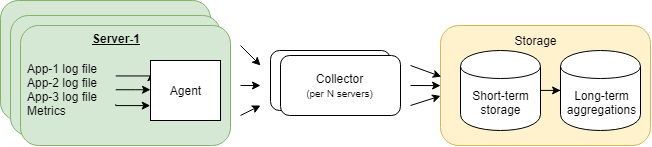
\includegraphics[width=0.9\textwidth]{figures/stateOfTheArt/logCollectionSchema.png}
    \caption{Log and metric collection schema.}
    \label{fig:sota_logCollection_schema}
\end{figure}

The main competitors are Splunk\footnote{\url{https://www.splunk.com/en_us/solutions/solution-areas/log-management.html}} Elastic ELK stack\footnote{\url{https://www.elastic.co/webinars/introduction-elk-stack}}. Out of some plugins, integrations and SDKs, both solutions have nearly the main functionality. The main difference is the format of data which is used for data storing\footnote{\url{https://devops.com/splunk-elk-stack-side-side-comparison/}}. Splunk storage is based on HDFS \cite{sanjay2003google, shvachko2010hadoop} style allowing users parse logs and search over them in their raw forms. On the other hand, ELK which is built on no-sql database Lucene, need more work to parse logs before they are stored. Another difference which is more interesting for managers is the pricing, even though Splunk has a small free-tier option, it’s general price cannot compete with ELK open-source built. 

Another rising star would be Kuberneties monitoring project Prometheus. Docker based architectures are becoming more and more popular so integrated logging solution replacing its old GELF protocol is s step the right way. But we also would like to give a quick shout out to all open-source monitoring software like Nagios, Icinga, OpenNMS, Cacti or Zabbix\footnote{\url{https://geekflare.com/best-open-source-monitoring-software/}}. All of them are providing excellent support your application and server monitoring with advance statistic features, but we do not have the recourses to cover all of them.

\subsubsection{2E2}

TBD

\section{Anomaly detection algorithms}

With just slight modifications and the right interpretation it is possible to use for anomaly detection most of the standard machine learning algorithm. In this section we cover both supervised and unsupervised algorithms, but keep in mind, unsupervised approach is more reasonable since there is no database with labelled log for every software, their mutations and possible combinations. There is also a special category of semi-supervised methods which expects only anomaly-less runtime behaviour as training set. We are also covering time series analysis since many machine variables can be studied in a form of a time series.

Most of the earlier algorithms are based in event/log key count matrix. The counts can be computed from a fixed window, a sliding window or a session window with different results and goals. This feature extraction is focused only on events represented by constant parts of log and relevant papers, we are discussing later, are forgetting variable parts of logs. Another main downside of this approach feature representation is also, it does not take in account the order of log events as it happened in the time. So some alter models and papers are then working with log key sequences and log key variable sequences instead.

\subsection{Supervised anomaly classification}

Supervised classification models are trained on labelled datasets with both normal and abnormal behaviour.  With more labelled data supervised anomaly detection is more accurate, unfortunately, such datasets are rare and if created by operators can be hard to maintain with complexity even higher than maintaining database of regular expressions for log patterns as we discussed in subsection \ref{ssec:sota_logging_logging}, but still it is worth to discuss these algorithms and models.
There are more methods than SVM and Clustering, which are covered in this subsection, that can be used for anomaly detection. For instance, Random forest or K-nearest neighbours would work really well for supervised classification, but we have not found them to be used in any research.

\subsubsection{Logistic regression and SVM}

Since logistic regression has hard time to work with linearly inseparable data, it is hard to use and not exactly useful for log classification. It is better to use kernel SVM as it is used in \cite{liang2007failure}.  Using sliding window, SVM can be use as online classifier with low computational resources to compute a classification, but retraining based on user interaction has to be done offline together with all labelled dataset. SVM model is also not so intuitive for anomaly reconstruction. 
\subsubsection{Decision trees}
Tree structure-based models are the most intuitive and easy to use models of machine learning methods. Decisions are based on attributes with the best information gain, we can image that structure as a tree with conditions in nodes and final classification in leaves. So, intuitively, adjustations to the model does not have to be done with full retraining as it is in the case of SVM models, but just by adding new conditions replacing the original leaves of the model followed by new classification leaves. For example, in \cite{chen2004failure} decision tree model is employed to diagnose failures in request logs.
\subsection{Unsupervised anomaly detection}

Compare to supervised methods which need large labelled datasets to train their model, unsupervised methods work with data which do carry any prior information and the models are based only on their statistical attributes. As it has already been said, unsupervised methods are more promising for real-world implementation since the is lack of labelled data and this is also the reason we will speak about them more deeply. 

\subsubsection{Log clustering}

Clustering is a base unsupervised method working with spacing in a given space. We would be able to cluster event/log count matrix, getting clusters of behaviour and classifying anomalies based on cluster size or threshold distance to the closest cluster, but the results would not be the best.

\cite{lin2016log} proposes two-phase cluster learning – initialization and online learning.  This procedure does not work with pure event/log key count matrix, instead it is transformed according the principle of normalized Inverse Document frequency, in this case it means Invers Event Frequency. Then Agglomerative hierarchical clustering is used for the initialization running creating two clusters – normal behaviour and anomalies. Following learning phase serves for cluster further adjusting, it is either added a cluster if distance is smaller than a threshold for following update or a new cluster is created.

The classification inherits label of the closest cluster is the distance is smaller than a threshold or is classified as an anomaly otherwise. Vector distance is an easy operation which can be employed for early anomaly detection and is still intuitive for out of the box understanding.

\subsubsection{PCA}

Principal component analysis is an old and powerful statistical approach proposed in 1901 by Karl Pearson. The main goal is to transform an original feature space into a feature space with smaller dimension maximizing variability of the original data. It helps us identify similarity between data and identify possible outliers by preserving major characteristic.

The same principal can be applied to log analysis. After applying PCA to event/log key count matrix all standard behaviour will be aligned along the first several principal components and on the other hand anomalies will take place fare from them. \cite{xu2009detecting} projects a single event/log key count vector $y$ according following equation:
\begin{equation}
\label{eq:sota_adetect_pca}
d_{y} = (1 – PP^{t})y
\end{equation}
, where $P = [ v_{1}, v_{2}, … , v_{k}]$ is a matrix of the first $k$ main components. Then if the distance $ d_{y}$ is bigger than a threshold, state represented by vector $y$ is classified as an anomaly. 

The paper selects the number of principle components enough high to cover 95\% of data variance and the threshold limit based on square prediction error with limit of 0.001. With increasing both variables we can decrease the number of false positive alarms but with cost of misclassification of some anomaly states. The proper setting is highly case sensitive and has to be estimate by experimenting.

Another problem which comes with PCA is, the methodology is sensitive to the data used for training and is not easily adjustable based on additional input. Also as we see in equation \ref{eq:sota_adetect_pca} event/log key count vector of a specific size is expected, which makes it harder to record events/log keys which were not present in the training data. We would rather recommend using PCA model for post problem analysis purposes.

\subsubsection{Invariant mining}

Invariant mining was for a long time one of the most promising model for log anomaly detection. The intuition behind software invariants relies on comes from software determinism, expecting, there are just a specific amount of ways to get from a state of a software to another one. Ultimately, invariant mining can recognise a linear dependency between logged actions in normal process execution.

To illustrate this problematic, take a look at simple process flow of a program in figure \ref{fig:sota_invMining_simpleProcess}. We can see that every process starts with establishing connection to a server. This part of an execution contains two different log keys, exactly one which says where it is connecting (log A) and unspecified number of messages showing the task has not been completed (log B). Than after successfully connected to a server, process retries a variable from it and based on its value process continues differently. The common to every normal execution is log announcing the connection has been successfully closed (log G).

\begin{figure}[h]
    \centering
    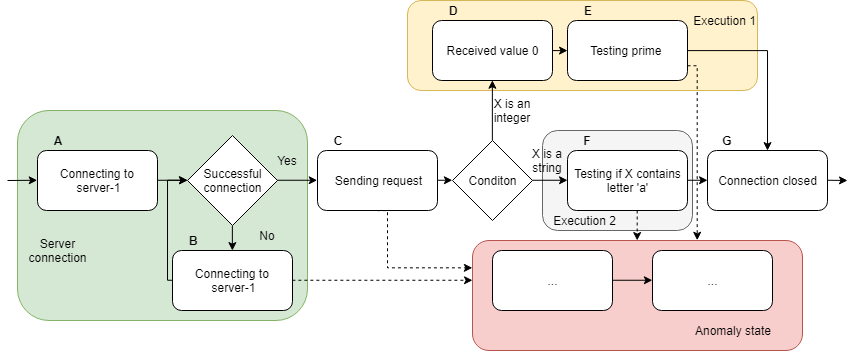
\includegraphics[width=0.9\textwidth]{figures/stateOfTheArt/simpleProcessWorkflow.png}
    \caption{Simple process diagram. Dashed connection stands for potential fatal exceptions.}
    \label{fig:sota_invMining_simpleProcess}
\end{figure}

For our case of a simple process flow, if the number of logs A is the same as the amount of logs G, there was not abnormality in whole execution. But, for instance, in case $sum(A) \neq sum(G)$ and $sum(A) = sum(C)$, we know that connection was successful and there was a problem further in the process execution. An advantage of invariant mining is its independency of specific executions since it searches for common rules. Intuitively, the same case would be, for instance, file open and close, connection and disconnection from a database, tcp protocol or message about timestamp parse failure followed by message about applying default timestamp. 

The first application of invariant mining is in \cite{lou2010mining} which uses singular decomposition on event/ log key count matrix to estimate the number of invariant, then it is followed by brute force mining algorithm to find potential linearities. As final invariant are marked only the couples which appear in more than 98\% of relevant event/log key count sessions.

Invariant mining is classified as unsupervised method, but it would be also fitting to between semi-supervised methods because it achieves much butter results if it is trained on data which do not contain any anomaly. In case, for than 2\%  of all training data are anomaly sessions, the original algorithm would not yield any invariant. It is possible to decrease the threshold and take $n$ estimated by the decomposition step most frequent invariant, but it is again a trade off with quality rapidly increasing potential false positive rate.

Even though invariants can be easily added if an adjustment is needed, invariant mining does not carry any information about event which happens between the related actions. It destines invariant mining to work mostly with session windows based created event/log key count matrix which can be hard to create for some application and systems. On the other hand, context execution to provide a reasoning behind a classification is based on un/fulfilled invariant. It makes it easy to understand.

\subsubsection{Workflow inference}

Workflow inference is natural follow up to invariant mining. CSight \cite{beschastnikh2014inferring} is an example of a framework which is half-way through to full workflow inference method. It mines invariants and uses them as input to counter-example guided abstraction refinement \cite{clarke2000counterexample}, so a basic workflow improves to a state in which it satisfies all of mined invariant. The result model is a communicating finite state machine \cite{brand1983communicating} and every execution which does not fits to the automata behaviour is classified as an anomaly.
The main step back of CSight is its requirement for users to select log pattern which should be considered, which again requires user domain knowledge and unnecessary interaction. As well as that training data have to contain multiple similar runs so invariants can be mined, but this is a problem inherited from invariant mining methodology.

The state of the art of workflow inference problematic is presented in CloudeSeek  \cite{joshi2017cloudseer}. It analyses log keys ordering in a log file and compresses it to multiple automates for different processes. Automate walk-through is triggered with every newly incoming log key and classified normal if at least one automata visited all states, with the difference to a classic walk-through, that the process can continue from any already visited state. In case there is no transition which is not satisfied by any edge of automates, anomaly alert is triggered.

We are using an example from the original paper to illustrate training process and classification of CloudSeek.  Let’s consider two sequences of log keys $ k_{1}, k_{2}$ and $ k_{1}, k_{3} $ which can be seen as that $k_{1}$ precedes $k_{2}$ and that $k_{1}$ precedes $k_{3}$. This behaviour can be transform to an automata displayed in figure \ref{fig:sota_workflowinference}, with starting states for $k_{x}$ being a collection of target states of edges labelled as $k_{x}$.

\begin{figure}[h]
    \centering
    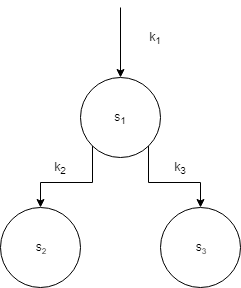
\includegraphics[width=0.4\textwidth]{figures/stateOfTheArt/cloudSeek_simpl_automata.png}
    \caption{Simple automata to illustrate workflow inference anomaly detection process.}
    \label{fig:sota_workflowinference}
\end{figure}

For the classification, let’s, firstly, consider a sequence $ k_{1}, k_{2}, k_{3} $. The walk-through triggered on $k_{1}$ starts in state $s_{1}$, then it is followed by $k_{2}$ which sets the set of states to continue to $[ s_{1}, s_{2}]$. The next incoming is $k_{3}$, with this log key the walk-through can proceed from $s_{1}$ to $s_{3}$, so no anomaly is identified and since all state have been visited walk-through ends. The other case happens for a sequence $ k_{2}, k_{1}, k_{3} $. Starting in state $s_{1}$ there is no edge we can move having following log key $k_{1}$ and anomaly warning is yield.

Workflow inference is, as well as invariant mining, on the edge between unsupervised and semi-supervised methods. The best result is achieved with training data of just normal behaviour, because then there is no chance, an automaton contains an edge which would satisfy anomaly behaviour. In case of training data with both behaviour types, a threshold for creating edges has to be set to avoid normalizing abnormal executions. Another possible for anomaly detection is heuristic based automata state classification, for instance error log keys. Then a warning can be also triggered earlier if the only possible walk-through leads to such state. On the other hand, automates are rather easy to modify based on additional inputs, which can make it easy for operators to adjust the model according their needs.

%\subsubsection{TDIDF}
%Used in \cite{zhang2016automated}

\subsection{Semi-supervised anomaly detection}
Up to now, we discussed methods which were either trained on labelled or unlabelled data containing for normal and abnormal behaviour. There are some methods which would work better with the requirement of semi-supervised learning – having only normal behaviour to train on, but the methods do not have that stated in their proposal. 

We understand, having strictly normal behaviour can be considered as a labelled dataset with no anomalies, but from the point of view of architecture operator, it makes a big difference. To create a labelled dataset with most of potential anomalies present and labelled in much harder than having a clear execution since a stable service does not experience problems so often.
\subsubsection{Long short-term memory}

LSTM \cite{hochreiter1997long} model implemented in DeepLog \cite{du2017deeplog} is the first neural network model we are discussing here and is currently the best solution to anomaly detection for software logs.  The intuition behind that approach is based on natural language processing (NLP), but instead of studying the content of separate log messages, it focuses at log key sequences works with log keys as with words. In every language we can identify rules and grammar and LSTM-based model expects the same for log sequences. In the end. we can see a log file as a way a software speaks to us.

The previously named work proved that and implemented an anomaly detection based on N-grams, but LSTM, which is an instance of recurrent neural networks (RNN), seems to be more promising, so we discuss only that here. General LSTM takes a vector of values and return probability distributing for values which can follow the input vector. An anomaly classification is assigned, if probability of truly following log key is not between the first some highest probabilities. Unfortunately, neural networks are more complex for formalization, so we are including formalization specific for log analysis and a figure \ref{fig:sota_lstm_deeplog} of used model from \cite{du2017deeplog}.

\begin{figure}[h]
    \centering
    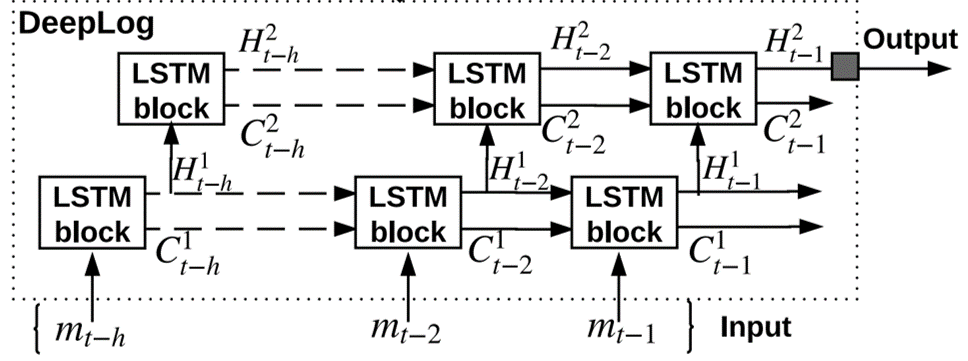
\includegraphics[width=0.9\textwidth]{figures/stateOfTheArt/deepLogLSTM.png}
    \caption{Visualization of LSTM used in DeepLog. Image used from \cite{du2017deeplog}.}
    \label{fig:sota_lstm_deeplog}
\end{figure}

Let’s expect we have a set of all $n$ possible log keys $K={ k_{1}, k_{2}, … , k_{n}}$. Then for training and classification we will be always working sliding windows sequences $w$ at a time $t$ of length $h$ denote as $ w_{t} = [m_{t-h}, m_{t-h+1}, … , m_{t-2}, m_{t-1}]$, where $m_{i}$ stands for $i^{th}$ log key of an input sequence of log keys. Having all this set, we can formalize model output of a conditional probability distribution as $Pr[m_{t} = (k \in K) |w_{t} ]$. 

In the figure \ref{fig:sota_lstm_deeplog} we can see that single $m_{i}$ of $w_{t}$ is an input to a single LSTM block and each block is also fed by a hidden vector $H_{t-i}$ and a cell state $C_{t-i}$ from the previous time step (block timely one step older). In this case, this composition is called deep LSTM and deeper layers of the network are fed by sequence of hidden vectors instead of log keys correspondently. 

There are 4 customisable parameters for such neural network ad decision process: 1) window size $h$ used as input vector, 2) number of layers/ depth of LSTM $L$, 3) amount of memory for each LSTM block $\alpha$ and 4) threshold $g$ saying how many highest log key probabilities are considered to be normal. The default setting of DeepLog is $h=10$, $L=2$, $\alpha=64$ and $g=9$. 

The framework is focusing on log key sequences and log key parameters separately using the same infrastructure. There is also a built-in functionality for feedback, which is adjusting weight within the neural network if an operator classifies alerted behaviour to be normal. This helps to improve the model with normal situations which were not present in the training set.

DeepLog can capture nonlinear and high dimension dependencies of system normal execution with high accuracy, but since neural networks works as a black box for users, there is just a little chance to provide more than alerting to operators. This is the reason why DeepLog also builds workflow model together with LSTM to give operator change to identify the root cause of the problem alerted by neural network.

\subsection{Comparison of classification methods}

All below listed algorithms are compared in table \ref{table:anomalyDetectionAlgs}. In the table you can also see efficiency of algorithms defined by precision, recall and f-measure. The values are taken from both papers for HDFS data and one for BGL data. We can see that for HDFS data supervised methods SVM and decisions trees performs really well, but for BGL, which has more complex execution and all anomalies are not present in training set, the performance lacks in recall and F-measure. From the unsupervised section we can see that invariant mining outperforms log clustering and PCA for both datasets in \cite{he2016experience} but the later work proved superiority of neural networks.

\begin{table}[h!]
\centering
\begin{tabular}{| >{\centering\arraybackslash}m{1.6cm} | c | c | c | >{\centering\arraybackslash}m{2.6cm} | >{\centering\arraybackslash}m{2.5cm} |} 
 \hline
 Algorithm & Type & Model update & Classifying & Efficiency \cite{he2016experience} HDFS/BGL & Efficiency \cite{du2017deeplog} HDFS \\ 
 \hline
 SVM & Sup. & Retraining & Online & 1-1-1/ 0.95-0.57-0.71 & - \\ 
\hline
 Decision tree & Sup. & Adjustable & Online & 1-1-1/ 0.95-0.57-0.72 & - \\
\hline
 Clustering & Unsup. & Retraining & Online & 0.87-0.74-0.8/ 0.42-0.87-0.57 & - \\
\hline
 PCA & Unsup. & Retraining & Online & 0.98-0.67-0.79/ 0.5-0.61-0.55 & 0.98-0.67-0.79\\
\hline
 Invariant mining & Unsup. & Adjustable & Sessions & 0.88-0.95-0.91/ 0.83-0.99-0.91 & 0.88-0.95-0.91\\
\hline
 Workflow inference & Unsup. & Adjustable & Online & - / -  & - \\
\hline
 LSTM & Semi-sup. & Adjustable & Online & - / - & 0.95-0.96-.0.96 \\
\hline
\end{tabular}
\caption[Machine learning algorithms used for anomaly detection with their efficiency.]{Machine learning algorithms used for anomaly detection with their efficiency describe by precision, recall and f-measure using \cite{he2016experience} and \cite{du2017deeplog}}
\label{table:anomalyDetectionAlgs}
\end{table}

\subsection{Time series analysis}

As we discussed in subsection \ref{ssec:sota_logging_monitoring}, general server monitoring produces mostly numeric time series, which are exactly fitting to the scope of time series analysis. But all the metrics do not have to serve just to problem detection. Another important mission is dynamic server provisioning and management \cite{ hong2011dynamic,chen2008energy}.

Being efficiently able to predict high workloads, performance peeks and gaps can limit expenses and also limit possible delays. There is a high requirement from companies to be able to scale up and down their services according current demand to take it maximally cost-effective.  According to \cite{barroso2007case}, 40\%-50\% of cost of running a high-performance computing platform is in its energy consumption. But this is not in scope of this thesis.

\subsubsection{ARMA models}

Autoregressive moving average models were introduces in 1954 by \cite{gurland1954hypothesis} and since the time there are many adaptations of the original work. ARMA model is represented and defined by order of its autoregression and moving average parts, but the main problem is it assumes stationarity of input series, but this is too strong assumption for real world data and also for variables which we can obtain from machine monitoring. 

\textbf{ARIMA} (AutoRegressive Integrated Moving Average) is the first generalization of the standard ARMA model to cover non-stationary numeric series introduced by \cite{ge1970box} in 1970. 

\textbf{SARIMA} (Seasonal ARIMA)

\textbf{ARFIMA} (Autoregressive Fractionally Integrated Moving Average)

\cite{kumar2016forecasting}
\cite{akouemo2017data}

\subsubsection{Singular Spectrum Analysis}

TBD
 \cite{kumar2016forecasting}
 
\subsubsection{Hierarchical temporal memory}

TBD
\cite{ahmad2016real}

\subsubsection{Artificial neural network}

TBD
\cite{akouemo2017data}


\chapter{Dataset}
\label{chap:dataset}

Datasets are important part of every research projects, you can either use it to evaluate your models or even train your models. Then the gold mind is every labelled dataset which provides the ground truth. The problem is that each dataset is really field specific so in our case we cannot use, for instance, a dataset of handwritten digits for our case. Another problem with the kind of data we need is that it can be really big. \cite{xu2009detecting} worked with Hadoop cluster logs generated in range of 48 hours by more than 200 nodes with total volume bigger than 200 TB, which were not, unfortunately, shared any further.

\section{Existing datasets}

Specific focus of this thesis limits us in what available dataset can be useful. The following list names the one we found:

\begin{itemize}

    \item \textbf{NAB\footnote{\url{https://github.com/numenta/NAB}}} - Numenta Anomaly Benchmark introduced in \cite{ahmad2017unsupervised} containes real-world and artificial time serias which can serve us for training time series monitoring based anomaly detection such we listed in part \ref{ssec:sota_logging_monitoring}. Especially data for AWS cloud watch which covers CPU utilization, network traffic and Drive I/O and time series from section Known causes with misconfiguration causing CPU problems and system failure resulting EC2 request latency.
    
    \item \textbf{ODDS\footnote{\url{http://odds.cs.stonybrook.edu}}} - Outlier Detection DataSets collects multiple different datasets for outlier/anomaly detection since 2016 from all the interest fields around. Even though we did not find any dataset which would 100\% fits to our research it can be useful for general testing of state clarification of anomalies. 
    
    \item \textbf{Loghub\footnote{\url{https://github.com/logpai/loghub}}} can provide a large collection of system logs per stand alone applications. This collection is cited and used by most of the recent papers and works dealing with system log parsing and analysing.

   \item \textbf{HDFS\footnote{\url{https://figshare.com/articles/HDFS_Logs/4040124}} \cite{xu2009detecting,xu2009online,Zhu2017}} contains log from more than 200 Hadoop nodes labelled by a Hadoop expert. There are about 2.9\% anomaly behaviour segments along more than 11 millions logged events total. This dataset was also used by many works we are refereeing in chapter \ref{chap:stateOfTheArt}.
    
\end{itemize}

\section{Our new dataset}

Unfortunately, none of the datasets listed above fully represents a complex software architecture by our definition of complex software architecture \ref{def:complexSoftwareArch}. We had a chance to create such dataset in cooperation with SAP Concur and discuss it in this section.

\subsection{Service architecture}

SAP concur has a team which is responsible for internal 

\subsection{Problems}

\subsection{Current alerting system}

\subsection{Log structure}









\begin{figure}[h]
    \centering
    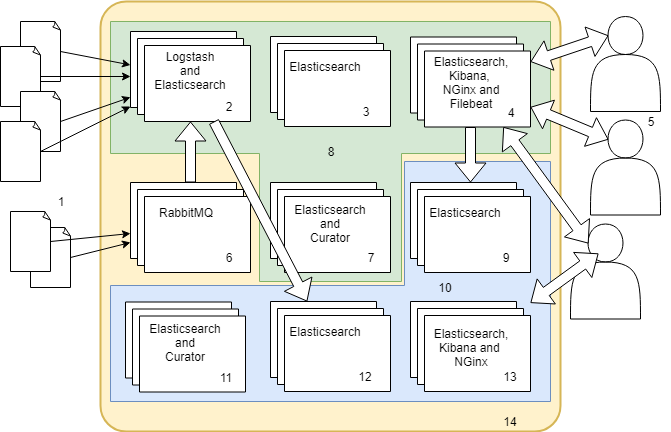
\includegraphics[width=0.9\textwidth]{figures/dataset/Parpr1Model.png}
    \caption[Illustration of a logging platform in one environment.]{Illustration of a logging platform in one environment. Explanatory notes: 1. incoming documents from users, 2. collector nodes with Logstash and Elasticsearch instance, 3. Elasticsearch data nodes of the green cluster, 4. servers running Kibana for log visualisation, 5. users, 6. RabbitMQ cluster, 7. Elasticsearch master nodes of the green cluster of the green cluster, 8. green cluster, 9. Elasticsearch ingests nodes, 10. blue cluster, 11. Elasticsearch master nodes of the blue cluster, 12. Elasticsearch data nodes of blue cluster, 13. servers running Kibana for log visualisation of the blue cluster, 14. logging platform environment setup}
    \label{fig:loggingPlatformIlustration}
\end{figure}
\chapter{Suggested solution}
\label{chap:solution}
\chapter{Experiments}
\label{chap:experiments}
\chapter{Conclusion}
\label{chap:conclusion}

%**************************************************************

\bibliographystyle{abbrv}
{
\def\CS{$\cal C\kern-0.1667em\lower.5ex\hbox{$\cal S$}\kern-0.075em $}
\bibliography{reference}
}

%**************************************************************

\appendix

\include{content/X_appendix.tex}
\end{document}
